\documentclass[11pt,letterpaper]{article}
\usepackage[utf8]{inputenc} %Codificacion del texto (ISO Latin1 encoding)

\usepackage{fancyhdr} %Permite acomodar a tu gusto la parte de arriba y
% abajo del documento
\usepackage[spanish]{babel} %Permite definir el idioma del dcumento
\usepackage{graphicx} %Permite exportar imagenes en formato eps
\usepackage{url} %Tipo de fuente para correos y paginas
\usepackage{pgf}
\usepackage{fleqn}
\usepackage{amssymb}
\usepackage{fancyvrb}
\usepackage{sectsty}
\usepackage{makeidx}
\usepackage{colortbl} %Permite colocar colores a las tablas
\usepackage{booktabs}
%%%%%%%%%%
%Margenes%
%%%%%%%%%%
\parskip 1mm %Espacio entre parrafos

\setlength{\topmargin}{0pt}

\oddsidemargin	0.5cm  % Ancho Letter 21,59cm
\evensidemargin 0.5cm  % Alto  Letter 27,81cm
\textwidth	15.5cm
\textheight	21.0cm
\headsep	4 mm
\parindent	0.5cm
%%%%%%%%%%%%%%%%%%%%%%
%Estilo del documento%
%%%%%%%%%%%%%%%%%%%%%%
\pagestyle{fancyplain}

%%%%%%%%%%%%%%%%%%%%%%%%%%%%%%%%%%%%%%%%%%%
%Fancyheadings. Top y Bottom del documento%
%%%%%%%%%%%%%%%%%%%%%%%%%%%%%%%%%%%%%%%%%%%
% Recuerde que en este documento la portada del documento no posee
% numeracion, pero de igual manera llamaremos a esa primera pagina la numero
% 1, y la que viene la dos. Esto es para tener una idea de las que
% llamaremos pares e impares
\lhead{Sistemas de Informaci\'on} %Parte superior izquierda
\rhead{\bf \it Tarea 2} %Parte superior derecha
\lfoot{\it Creando Organizaciones para el Futuro} %Parte inferior izquierda. \thepage indica
% el numero de pagina
\cfoot{} %Parte inferior central
\rfoot{\bf \thepage} %Parte inferior derecha
\renewcommand{\footrulewidth}{0.4pt} %Linea de separacion inferior

% Challa

\newtheorem{theorem}{Theorem}
\newtheorem{acknowledgement}[theorem]{Acknowledgement}
\newtheorem{algorithm}[theorem]{Algorithm}
\newtheorem{axiom}[theorem]{Axiom}
\newtheorem{case}[theorem]{Case}
\newtheorem{claim}[theorem]{Claim}
\newtheorem{conclusion}[theorem]{Conclusion}
\newtheorem{condition}[theorem]{Condition}
\newtheorem{conjecture}[theorem]{Conjecture}
\newtheorem{corollary}[theorem]{Corollary}
\newtheorem{criterion}[theorem]{Criterion}
\newtheorem{definition}[theorem]{Definition}
\newtheorem{example}[theorem]{Example}
\newtheorem{exercise}[theorem]{Exercise}
\newtheorem{lemma}[theorem]{Lemma}
\newtheorem{notation}[theorem]{Notation}
\newtheorem{problem}[theorem]{Problem}
\newtheorem{proposition}[theorem]{Proposition}
\newtheorem{remark}[theorem]{Remark}
\newtheorem{solution}[theorem]{Solution}
\newtheorem{summary}[theorem]{Summary}
\newenvironment{proof}[1][Proof]{\noindent\textbf{#1.} }{\ \rule{0.5em}{0.5em}}

\newcommand{\primaria}[1]{
	\textbf{\underline{#1}}
}

\newcommand{\foranea}[1]{
	\textbf{\textsl{#1}}
}

\newcommand{\primyfor}[1]{
	\underline{\foranea{#1}}
}

\makeatletter
\newcommand\subsubsubsection{\@startsection {paragraph}{1}{\z@}%
                                   {-3.5ex \@plus -1ex \@minus -.2ex}%
                                   {1.5ex \@plus.2ex}%
                                   {\normalfont\bfseries}}
\newcommand\subsubsubsubsection{\@startsection {subparagraph}{1}{\z@}%
                                   {-3.5ex \@plus -1ex \@minus -.2ex}%
                                   {1.5ex \@plus.2ex}%
                                   {\normalfont\bfseries}}


\makeatother

%\makeindex
%%%%%%%%%%%%%%%%%%%%%%%%%%%%%%%%%%%%%%%%%%%%%%%%%%%%%%%%%%%%%%%%%%%
%%%%%%%%%%%%%%%%%%%% Aqui empieza el documento %%%%%%%%%%%%%%%%%%%%
%%%%%%%%%%%%%%%%%%%%%%%%%%%%%%%%%%%%%%%%%%%%%%%%%%%%%%%%%%%%%%%%%%%

\begin{document}

%%%%%%%%%%%%%%%%%%%%%%%%%%
%Definicion de la portada%
%%%%%%%%%%%%%%%%%%%%%%%%%%
\begin{titlepage}
    \begin{center}
	\begin{tabular}{ccc}
	    %\epsfig{file=escudo-utfsm.eps, height=1.6cm}
	      
\includegraphics[height=1.6cm]{images/logoUTFSM}
	    & %Escudo de la Universidad Santa Maria
	    \hspace{0.2cm}
	    \begin{tabular}{c}
		Universidad Técnica Federico Santa María \\ \hline
		\hspace{8.0cm}
		\vspace{1.2cm}
	    \end{tabular}
	    \hspace{0.2cm}
	    &
	   % \epsfig{file=logo_DI.eps, height=1.6cm} %Logo del DI
            
\includegraphics[height=1.6cm]{images/logoDI}
	\end{tabular}

	\vspace{2.5cm}
	%Titulo del Documento
	    \begin{tabular}{c}
		\Huge{\textbf{Tarea 2}}\\\\\\\\\\\\\\
		\LARGE{\textbf{``Sistema de Gesti\'on de Clientes VIP''}}\\\\
		\LARGE{\sc{Fundamentos de Ingenier\'ia}}\\
		\LARGE{\sc{de Software}}
	    \end{tabular}

	\vspace{2.5cm}
%	\begin{tabular}{c}
	\begin{center}
%	     \pgfimage[height=1.8cm]{images/now}
	%    \Huge{\emph{Now!}}
%	\end{tabular}
	\end{center}
	
        \vspace{1.5cm}

	%Nombre del (o los) autor(es)
	\begin{tabular}{lr}
            \begin{tabular}{c}
	        \large{Rodrigo Fern\'andez - 2673002-3}\\
		\large{\url{rfernand@inf.utfsm.cl}}
	    \end{tabular}
	&
	   \begin{tabular}{c}
         	\large{Cristi\'an Maureira - 2673030-9}\\ 
		\large{\url{cmaureir@inf.utfsm.cl}}
	   \end{tabular}
	\end{tabular}
        \vspace{3.5cm}\\
	%Fecha
		\large{\sc{Valpara\'iso, Octubre 2008.}}
    \end{center}
\end{titlepage}


\section*{\'Indice}
\label{sec:indice}
\vspace{2cm}
\begin{itemize}
	\item Introducci\'on       \hspace{10cm}    P\'ag. 02\\
	\item S\'intesis del Texto \hspace{9.15cm}  P\'ag. 03\\
	\item Rese\~na del Autor   \hspace{9.19cm}  P\'ag. 05\\
	\item Apreciaciones        \hspace{9.83cm}  P\'ag. 06\\
	\item Conceptos            \hspace{10.4cm}  P\'ag. 08\\
	\item Conclusi\'on         \hspace{10.3cm}  P\'ag. 10\\
	\item Referencias          \hspace{10.25cm} P\'ag. 13\\
	\item Glosario             \hspace{10.75cm} P\'ag. 13\\
	\item M\'etodo de Trabajo  \hspace{8.9cm}   P\'ag. 13\\
\end{itemize}
\vspace{5cm}


\section*{Introducci\'on}
\label{sec:introduccion}
Cuando ni\~nos nos ense\~nan que la comunicaci\'on es el acto de entregar y recibir datos entre
personas, conversar acerca del clima, preguntarnos como nos ha ido en el d\'ia, saludarnos para los
cumplea\~nos, escribirnos correos, llamarnos por tel\'efono, etc. y desde entonces hemos dado por
sentado sin un menor esfuerzo por indagar al respecto que en eso se agota la comunicaci\'on. Nos
desenvolvemos en un mundo en el que al parecer la relevancia de los actos lingu\'isticos quedan en
un segundo plano donde se le atribuye tan s\'olo el m\'erito de permitir a los humanos expresarse e
intercambiar ideas y sentimientos. Parece una percepci\'on bastante razonable, sin embargo veremos 
que la comunicaci\'on a trav\'es del lenguaje implica una construcci\'on de la realidad en esa acci\'on
 de entregar y recibir datos.\\

En el presente informe abordaremos temas presentes en el texto de Fernando Flores como
la Teor\'ia de la Acci\'on y los respectivos conceptos que la conforman como el lenguaje, las peticiones y
promesas, y las conversaciones que dentro de \'este se dan. Destacaremos la importancia que tienen
acciones simples como escuchar para colaborar y planificar siendo creativos para el buen funcionamiento
 de empresas y organizaciones en general. Caeremos en la cuenta de que la comunicaci\'on
es en la pr\'actica un sistema de informaci\'on.\\

Estudiaremos el concepto de "Workflow" (Flujo de Trabajo) demostrando que la coordinaci\'on
de masas se realiza a trav\'es de la conversaci\'on. Veremos como los estados de \'animo y emociones
juegan un papel absolutamente importante en el dise\~no de las organizaciones. Profundizaremos
acerca del acto de escuchar, que hoy en d\'ia creemos entender pero no siempre lo entendemos del
todo.\\

Retomaremos lo estudiado previamente en "La Quinta Disciplina" por Peter Senge, donde
aprendimos que el aprendizaje en una organizaci\'on es totalmente imprescindible y debe ser constante
 y permanente en el tiempo, de modo que nuestra empresa cumpla sus objetivos globales y
los de sus miembros.
\vspace{5cm}


\section*{S\'intesis}
\label{sec:sintesis}
Los seres humanos viven en organizaciones, en el d\'ia a d\'ia nos envolvemos en un trabajo que es posible gracias a marcos organizacionales. El ser social m\'as significativo es un comportamiento organizacional. Lamentablemente no se comprende que es una organizacion, ni su dise~no y en que pueden evolucionar. Las persona que se envuelven en organizaciones no act\'uan de manera creativa a los problemas que se le presentan y se resignan ante el fracaso de algun proyecto organizacional. La respuesta es de \'ambito intelectual como pr\'actico. \\ 

Una organizaci\'on se define como un lugar donde se generan conversaciones, las cuales son fen\'omenos sociales en los que se realizan trabajos como toma de desiciones, formacion de juicios y manejo de posibilidades. Las organizaciones son el producto de las conversaciones y no viceversa. \\ 

Para la definici\'on de una organizaci\'on debemos declarar ciertos oficios que cubran el amplio campo de las conversaciones y posibles movimientos de ellas, ademas de definir quien esta facultado y tiene el deber de realizar los oficios. \\

Estas declaraciones en s\'i no son los objetivos o metas, sin embargo, las organizaciones estan basadas en conversaciones, tanto recurrentes como de un trasfondo espec\'ifico y compartido. \\

Las organizaciones deben plantearse proyectos espec\'ificos, los cuales poseen un camino abierto gracias a la declaraci\'on de su dominio de posibilidades. Estos proyectos requieren un lenguaje de acci\'on y condiciones de satisfacci\'on para su realizaci\'on. \\

	CondicionesSatisfechas($accion_1$, $accion_2$, ..., $accion_n$)\\

La estructura interna de una organizaci\'on no basta con ser representada por un organigrama, sino que se deben especificar las relaciones entre las personas, las cuales consisten en compromisos lingu\'isticos entre ellas. Estos compromisos implican peticiones, promesas, declaraciones o afirmaciones entre personas, descubriendo de esta forma la estructura real de una organizacion. \\

En una organizaci\'on el poder se encuentra localizado, lo que implica problemas si es que en un sector se ubica la tarea de crear y administrar las conversaciones y en otro sector el declarar el \'ambito de posibilidades para la organizaci\'on, debido a que puede ocurrir que las acciones demandadas no se encuentren en entre las posibilidades declaradas. Lo importante es tener en cuenta las declaraciones a nivel operacional y no las que se anuncian para una acci\'on especifica, adem\'as de tener presente de que posibilidades permite la estructura de la organizaci\'on para ejecutar el poder, que posibilidades de poder existen considerando a la organizacion con su entorno, historia, cultura y pol\'itica, posibilidades de poder tiene la organizaci\'on considerando su pasado o herencia y su futuro o destino. \\

La emoci\'on es m\'as que un fen\'omeno natural. Las emociones definen nuestro estado de \'animo, debido a \'esto, se produce un fen\'omeno lingu\'istico que conlleva a producir variaciones en nuestro espacio de posibilidades frente al futuro. El estado de \'animo y juicios expanden o restringen la gama de conversaciones que podemos establecer con otras personas. Estas posibilidades de apertura y cierres se producen al escuchar. \\

Es esencial, si vamos a dirigir nuestras vidas y nuestras organizaciones como posibilidades, que escuchemos los estados de \'animo, las emociones y los juicios como aperturas y cierres de posibilidades sociales. \\

\vspace{14cm}


%inicio desarrollo

\section*{Rese\~na del Autor}
\label{sec:autor}
\textbf{Fernando\ Flores\ Labra}\\\\
\emph{Talca, 9 de enero de 1943}\\
Pol\'itico, fil\'osofo e ingeniero chileno, ex ministro de estado y actual senador de la Rep\'ublica.\\
Ingeniero comercial, doctor en filosof\'ia del lenguaje de la Universidad de Berkeley, fue ministro en dos
ocasiones del Presidente Salvador Allende y sufri\'o tres a\~nos de c\'arcel como preso pol\'itico durante
el r\'egimen de Augusto Pinochet por su participaci\'on en el gobierno de la Unidad Popular y su militancia Mapu.\\
Tras su liberaci\'on se instal\'o en California, Estados Unidos, donde desarroll\'o una intensa actividad acad\'emica
y empresarial.\\
Actualmente se desempe\~na como senador por la I Regi\'on de Tarapac\'a, por el período 2002-2010.\\
El 6 de noviembre de 2006, solicit\'o la suspensi\'on de su militancia del Partido por la Democracia (PPD), producto
de la -a su juicio- defensa que el partido le habr\'ia otorgado al senador Guido Girardi, tras el descubrimiento de la
entrega, por parte de \'este \'ultimo, de informaci\'on falsa al Servicio Electoral (Servel) respecto a sus gastos de
campa\~na en la \'ultima elecci\'on parlamentaria. El 9 de enero de 2007 present\'o su renuncia al partido.\\
En sus trabajos Flores plantea que gran parte de la coordinaci\'on humana ocurre en lo que denomin\'o "conversaciones
para la acci\'on", a trav\'es de las solicitudes, de las promesas y del cumplimiento de los compromisos entre las personas,
y sostuvo que la importancia de los computadores consiste en facilitar este trabajo de coordinaci\'on más que en el simple
procesamiento de datos.\\
Es fundador del Movimiento Atina Chile y Chile Primero (partido pol\'itico en formaci\'on) y corresponsal en diarios ciudadanos
como El Morrocotudo y El Rancahuaso.\\
Sus an\'alisis sobre las organizaciones humanas y el papel de la tecnolog\'ia desembocaron en diversos libros y en la creaci\'on
de empresas que desarrollaron software para la coordinaci\'on del trabajo en las organizaciones.\\
Entre sus obras destaca Understanding Computers and Cognition - A New Foundation for Design, publicado en 1986 junto a T. Winograd.\\
\begin{center}
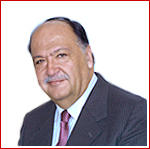
\includegraphics[height=3cm]{images/flores}
\end{center}
\begin{itemize}
	\item http://www.fernandoflores.cl
	\item http://www.chileprimero.cl
	\item http://www.atinachile.cl
\end{itemize}


\section*{Apreciaciones}
\label{sec:apreciaciones}
\begin{itemize}
	\item ?`Qu\'e diferencias existen entre organizaciones y conversaciones?

No existe duda que las organizaciones son fen\'omenos pol\'iticos, pero como bien sabemos que las organizaciones
son el producto de conversaciones, acciones y demases. Por ende Las organizacione tambi\'en producto de nuestras
conversaciones sobre como tendremos conversaciones acerca del contexto social (instituciones, oficinas, reglamentos,
etc) dentro del cual sostendremos conversaciones.
?`Pero es f\'acil poder distinguir que conversaciones son pol\'iticas?

Con algunos t\'erminos pol\'iticos como Democracia, Socialismo, Monarqu\'ia, etc, van a se\~nalar la posici\'on uno puede tomar con
respecto a alg\'un hecho, es decor, el camino que va a seguir la conversaci\'on organizacional. Si pudiesemos comprender todos los
t\'erminos, podriamos saber a trav\'es de ciertas declaraciones, como se transmite la fuerza de la acci\'on de la persona que las
emite, aparte de quienes pueden participar en ciertas conversaciones relacionadas con los t\'erminos anteriormente se\~nalados.
Si adoptamos \'estas posiciones, producimos los arreglos sociales esenciales para las conversaciones que podemos tener a futuro.
Tenemos que tener presente la idea de que somos todos parte de las conversaciones pol\'iticas, herando declaraciones que ya se han
dicho, por lo cual sabemos como se han desarrollado dichas conversaciones en nuestra sociedad.
Finalmente me gustaria compartir \'este parrafo, con el cual flores, nos deja se\~nalado como las conversaciones se convierten en un
ciclo que nosotros misnos formamos y aportamos:\\

\begin{center}
\emph{Incluso, cuando nuestra tarea es producir una organizaci\'on nueva, vale decir, una nueva compa\~n\'ia
o incluso una organizaci\'on pol\'itica del Estado enteramente nueva, nosotros s\'olo nos volvemos a unir a una conversaci\'on en la cual ya hemos
participado en calidad de escuchadores. De este modo el dise\~no de las organizaciones nunca parte completamente de nuevo.}
\end{center}

	\item El fenomeno ling\"uistico\\\\
 Es curioso como Fernando Flores se dio cuenta que del conversar (en el contexto organizacional) nac\'ia absolutamente todo.\\
 Encontramos que su forma de ver las cosas, el identific\'o que la organizaci\'on no es un conjunto de individuos sino una red
 de conversaciones, es bastante \'util y cierto. Especialmente, porque constituye que la empresa sustancialmente no son seres 
humanos, sino redes de conversaciones entre ellos. Es decir, de esta forma podemos identificarlas como redes de compromisos 
ling\"u\'isticos, redes de actos del habla que nos permiten estudiar mas a fondo las distintas interacciones que los representan
 en realidad. Esta postura, encontramos que es muy interesante de analizar, ya que sustenta la conversaci\'on como ``la unidad 
m\'inima de interacci\'on social orientada hacia la ejecuci\'on con \'exito de acciones''. De este modo,
 la conversaci\'on se convierte en un fen\'omeno clave en las organizaciones, partiendo de la base que el lenguaje es invenci\'on y 
constituci\'on de realidad. El \'enfasis del concepto est\'a centrado en la comunicaci\'on para la acci\'on. Y gracias a esto, uno
 puede darse cuenta de como para entender una organizac\'ion (o conocerla realmente), es m\'as relevante estudiar las diferentes redes
 de conversaciones que ven resultados concretos, sin importar el tipo de empresa o organizacion, ya sea en \'ambitos de los negocios,
 de la educaci\'on, del tiempo libre, de las finanzas o de la pol\'itica.\\

As\'i, compartimos la opinion que el lenguaje, m\'as que ser una herramienta descriptiva, se vuelve una pr\'actica articuladora de los
 diferentes procesos que se llevan a cabo. El que el lenguaje forma un constructor de realidad y forma en que la historia se manifiesta.
 A pesar de no ser algo muy facil de comprender, tambien entendemos que nada ocurre dentro de la organizaci\'on sin el lenguaje. Sin 
lenguaje no podr\'iamos construir organizaciones. A trav\'es de \'el, los individuos se transforman en miembros del entorno ps\'iquico 
de la organizaci\'on. La piensan desde all\'i y logran definirla en su totalidad.\\

	\item Sobre su pensamiento

Se entiende de que Fernando Flores  no est\'a interesado en la organizaci\'on en s\'i, 
como un ente, por el contrario hace referencia a los problemas que se producen en la realizaci\'on y dese~no del trabajo.

Flores se~nala un pensamiento, que da el pie inicial sobre una nueva visi\'on al analizar las organizaciones, como una especie de redes de compromisos entre las personas que las componen, las cuales se atribuyen a acciones de caracter lingu\'istico.

Tambi\'en menciona una definici\'on para los tipos de procesos que definen el funcionamiento de las organizaciones: \\

Un proceso de producci\'on, en donde se refiere a transformar y unir las materias primas en componentes y productos. \\ \\
Luego se refiere a la producci\'on de informaci\'on, el cual consiste en manipular, comunicar y despleguar eventos y procesos referentes al negocio. \\ \\
Por \'ultimo hace referencia a un proceso de satisfacci\'on al cliente, el cual se refiere a realizar y completar condiciones de satisfacci\'on entre los clientes y el que provee.

\end{itemize}
\vspace{5cm}


\section*{Conceptos}
\label{sec:conceptos}
\begin{enumerate}
	\item Escuchar

Flores se\~nala que si una persona establece en una conversaci\'on de que puede
 ocurrir un problema si no se toma alguna desici\'on anticipada, este problema
 es algo subjetivo en la persona, aun cuando puede que otra persona no interprete
 en su escuchar un aparente problema.

Hablar y escuchar son fen\'omenos ricos segun Flores. Esto debido a que una
 persona si bien puede esta comunic\'andonos algun tipo de informaci\'on,
 nosotros obviamente lo escuchamos, pero a su vez el tambien se escucha, 
lo que implica que tiene en cuenta todas las cosas que el traspaso de esta
 informaci\'on significa, ya sea compromisos de hacer algo nuevo o compromisos
 personales para la realizaci\'on de ello. El escuchar implica el transfondo 
de cualquier cosa que le ocurra.

En momento en que se hace presente el acto de hablar es apenas la punta del 
iceberg en relaci\'n con este trasfondo. Esto implica compromisos espec\'ificos
 y expl\'icitos que el que comunica puede haber adquirido respecto a la nueva
 tarea que se gener\'o o generara, resultado de la informaci\'on que comunic\'o.


	\item El fen\'omeno ling\"u\'istico en las organizaciones

Seg\'un Fernando Flores, en las organizaciones, todo ocurre en base al
lenguaje, o dicho de mejor modo, a las conversaciones.\\
En toda conversaci\'on, alguien hace una petici\'on y la contraparte
(recordemos que en una conversaci\'on participa m\'as de una persona) realiza
una promesa, adecu\'andose a la petici\'on mediante las bien llamadas
``condiciones de satisfacci\'on''. Nada de esto ocurre sin el lenguaje, sin hablar y
escuchar. La organizaci\'on misma no existir\'ia sin el lenguaje, sin que alguien la
haya propuesto, anunciando p\'ublicamente su existencia.\\

Es de vital importancia aclarar qu\'e es lo que realmente se entiende por
lenguaje, por lenguaje entendemos conversaci\'on, pero para ser m\'as precisos,
``conversaciones para la acci\'on'' y ``conversaciones de posibilidades''. Pero
entonces, ?`qu\'e entendemos por conversaciones para la acci\'on?. Las
conversaciones para la acci\'on son aquellas mediante las cuales logramos que
las cosas se realicen, a diferencia de las conversaciones de posibilidades, las
cuales surgen a ra\'iz de las conversaciones para la acci\'on.\\

Al hacerse la petici\'on con su correspondiente promesa, aparece lo que
denominamos ``condiciones de satisfacci\'on'', que no es otra cosa que las
condiciones bajo las que se cumplir\'a una petici\'on o una promesa.
En lo que va del texto ya hemos profundizado dos grandes conceptos
que son posibles distinguir en las conversaciones para la acci\'on. Ahora se
ver\'an otros dos conceptos: las afirmaciones y las declaraciones.\\

Con una afirmaci\'on se dice que algo es as\'i o verdadero, una declaraci\'on,
por el contrario, no es decir que algo es as\'i: es hacer que sea as\'i. Las
conversaciones para la acci\'on comprometen a actuar; en cambio las conversaciones
 para posibilidades producen oportunidades para comprometerse en una acci\'on.\\

	\item El rol de la planificaci\'on

Dado que las organizaciones deben estar preparadas para cualquier eventualidad futura, \'estas
deben realizar extensos y rigurosos procesos de planificaci\'on para poder responder de la mejor
manera a las inclemencias del futuro. Hoy en d\'ia planificar significa prever, hacer predicciones y
estimaciones acerca de los d\'ias venideros a tal punto que nos preparamos para un futuro que creemos
va a suceder inminentemente. En este proceso lamentablemente estamos dejando de innovar.\\

No nos referimos a innovar como un proceso de descubrir una f\'ormula del \'exito completamente
revolucionaria. La creatividad en este caso pasa por un asunto de saber escuchar posibilidades
para nuestra organizaci\'on de avanzar hacia el desarrollo. Muchas veces empresas con gran
capacidad t\'ecnica y buenos profesionales no triunfan por el simple hecho de que no saben extraer
de la realidad el camino a seguir. Un contra ejemplo al respecto es el siguiente: empresas como
Apple Computer sin tener mayores ventajas en avances tecnol\'ogicos (los mismos que su competencia
en aquel tiempo) termin\'o siendo un gigante de la computaci\'on personal a nivel mundial \'unicamente
gracias a la visi\'on emprendedora de sus miembros. Vale decir, supieron escuchar.\\

Como mencionamos, la comunicaci\'on se puede representar como un sistema de informaci\'on
en el cual las peticiones y ofertas son los mensajes que se env\'ian los distintos componentes. En
este caso los componentes son personas y las interacciones que se dan entre ellos corresponden a
conversaciones.



\end{enumerate}
\vspace{8cm}


%fin desarrollo

\section*{Conclusiones}
\label{sec:conclusiones}
En primera instancia, podemos concluir que las organizaciones no son entidades est\'aticas
que nos permiten relacionarnos para lograr nuestros deseos individuales y/o grupales. M\'as bien,
una organizaci\'on es un conjunto de consensos sociales definidos bajo el contexto de nuestra propia
historia, es decir, son declaraciones lingu\'isticas que recopilan pensamientos acordes a la \'epoca
en que se viva. Lo que tuvo sentido hace 1000 a\~nos ya no lo tiene, por tanto la definici\'on de una
organizaci\'on est\'a sujeta a constantes cambios. La gracia est\'a en poder llegar a la ra\'iz de lo que se
entiende por organizaci\'on para as\'i poder redise\~narlo de acuerdo al contexto, o lo que menciona el
texto como ``reconstrucci\'on ontol\'ogica''.\\

Se entiende que una organizaci\'on es un fen\'omeno pol\'itico, enti\'endase como un fen\'omeno
dado por la conversaci\'on social, referida a lograr los deseos propios y globales. Luego una organizaci\'on
es una conversaci\'on, pero no viceversa.\\

El hilo conductor dentro de una organizaci\'on es el lenguaje, sin \'el, nada podr\'ia acontecer, es
por esto que se debe comprender las estructuras de lenguaje dado un cierto contexto. Enti\'endase
al lenguaje como una dicotom\'ia, es decir, un constante hablar y escuchar, donde se reconocen partes
b\'asicas como la petici\'on que es respondida por la promesa, ya sea de una acci\'on o de una posibilidad.\\

 El escuchar no se refiere a ``o\'ir'' lo que pasa a mi alrededor, sino m\'as bien, a la percepci\'on y
juicio que yo pueda emitir dado el contexto en el que me desenvuelvo. Haciendo esta parte del
lenguaje en la persona como individuo que ha sido criado con ciertos patrones de entendimiento.\\

Todo este proceso es inmensamente rico en dos extremos opuestos: el trasfondo en que se
desarrolla (historia) y las posibilidades que se dan (pensamiento individual, donde influyen los juicios
 sociales).\\

%       Apreciaciones Personales

El texto presenta bastantes apreciaciones de \'indole filos\'ofica, mencion\'andose a grandes
nombres como Heidegger, del cual poca informaci\'on poseemos. Este matiz permite dar un espectro
 m\'as grande de explicaci\'on del pensamiento de Flores, dado que no est\'a creando ideas nuevas,
sino que se apoya en criterios ya hechos y probados para generar una nueva apreciaci\'on.\\

Se puede ver que las personas estamos mal enfocadas en muchos aspectos de nuestro pensar,
 dado que es muy dogm\'atico desde que somos ni\~nos. Nos forman de ciertas maneras con ciertas
estructuras mentales que luego hacemos propias y no podemos romper, de ah\'i que aceptemos
un ambiente de trabajo desagradable o un bajo sueldo, creemos que as\'i es la organizaci\'on pues
nunca nadie nos ense\~n\'o como se defin\'ia y por ende no podemos redise\~narla. Esto tiene directa
relaci\'on con el texto ``La quinta disciplina'' donde se mencionan los modelos mentales.\\

Finalmente podemos apreciar que Flores ha extendido a Senge agregando a su comprensi\'on
de la organizaci\'on la arista del lenguaje.\\

Nos pareci\'o un texto realmente interesante en todo aspecto. Rescata aspectos de la vida
que son cotidianos y que la mayor\'ia del tiempo no reparamos en su importancia. Sin duda una recopilaci\'on
de escritos que a m\'as de un miembro de directorio le debe haber abierto los ojos, ya
que si bien los temas metalingu\'isticos suelen ser dif\'iciles de entender, hay una verdad de fondo que
es indiscutible: nada ocurre en las organizaciones sin el lenguaje, hablar y escuchar es una tarea
fundamental.
\vspace{15cm}


\section*{Referencias}
\label{sec:referencias}
\begin{itemize}
	\item Creando Organizaciones para el Futuro, Fernando Flores.
	\item Wikipedia, la enciclopedia libre
\end{itemize}


\section*{Glosario}
\label{sec:glosario}
\begin{itemize}
	\item \emph{Conversaci\'on:} Proceso lingu\'istico en donde alguien hace una petici\'on y la contraparte
		realiza una promesa, adecu\'andose a la petici\'on mediante las bien llamadas “condiciones de satisfacci\'on”.
		Nada de esto ocurre sin el lenguaje, sin hablar y escuchar.
	\item \emph{Condiciones de Satisfacci\'on:} Son aquellas condiciones a cuales se somete el cumplimiento de una promesa
		o petici\'on, acordada en una conversaci\'on.
	\item \emph{Afirmaci\'on – Declaraci\'on:} Afirmaci\'on, es darle el valor de verdad a algo dicho, en cambio, declaraci\'on
		no apunta a decir como son las cosas, sino a hacer que sean de esa forma.
	\item \emph{Teor\'ia de la Acci\'on:} Teor\'ia que afirma que toda acci\'on humana esta precedida por actos lingu\'isticos
		que la determinan.
	\item \emph{Workflow:} Flujo de Trabajo. Secuencia de procesos industriales, administrativos u otros a trav\'es de los cuales
		una tarea pasa de ser iniciada a ser completada
	\item \emph{Retroalimentaci\'on:} Informaci\'on acerca de las reacciones de un individuo ante un est\'imulo. Usado como
		base para mejoras.
	\item \emph{Metalingu\'istico:} Lenguaje que se usa para explicar o hablar del lenguaje mismo.
\end{itemize}


\section*{M\'etodo de Trabajo}
\label{sec:metodo}
Para poder desarrollar \'este informe, nuestro grupo ley\'o de forma individual el Texto, record\'ando las apreciaciones
personales de los aspectos que mas llamaron la atenci\'on de la lectura.\\
Luego nos juntamos un par de d\'ias para discutir sobre lo entendido y los temas que definimos con mayor relevancia
fueron puesto en el texto, en la secci\'on correspondiente. Luego cada uno comenzo a redactar las ideas para luego poder
unir todos los documentos y formar el desarrollo central del trabajo.\\
Cada uno a medida que le\'ia el texto, ten\'ia como deber, anotar las palabras que no supiera o definiciones que encontrara
interesantes, para poder redactar el Glosario.\\
Finalmente, redactamos la introducci\'on y conclusi\'on general del trabajo realizado.


\end{document}
